
%(BEGIN_QUESTION)
% Copyright 2006, Tony R. Kuphaldt, released under the Creative Commons Attribution License (v 1.0)
% This means you may do almost anything with this work of mine, so long as you give me proper credit

Match the following operational amplifier circuits with their respective transfer functions from the list below (note that more than six functions are listed, just to make it more challenging!):

$$\includegraphics[width=15.5cm]{i01466x01.eps}$$

Note -- all the resistors labeled $R$ are the exact same value.  The $k$ appearing in some of the equations represents a ``programmable'' constant:

\vskip 10pt

$y = -kx$ \hskip 50pt $c = -(a + b)$ \hskip 50pt $y = 2x$ \hskip 50pt $y = x$ \hskip 50pt $y = -x$ 

\vskip 10pt

$c = a + b$ \hskip 50pt $y = kx$ \hskip 70pt $c = 2(a + b)$ \hskip 30pt $y = x \div k$ \hskip 30pt $c = a - b$ 

\vskip 20pt \vbox{\hrule \hbox{\strut \vrule{} {\bf Suggestions for Socratic discussion} \vrule} \hrule}

\begin{itemize}
\item{} Identify the ``simplifying assumptions'' we generally use when analyzing DC opamp circuits.  Hint: one has to do with the effect of negative feedback on the input voltages, and another has to do with the input terminal currents.
\item{} Explain {\bf why} each circuit perform its respective mathematical function!
\item{} Explain where the negative sign comes from in some of the circuits' equations.
\end{itemize}

\underbar{file i01466}
%(END_QUESTION)





%(BEGIN_ANSWER)

$$\includegraphics[width=15.5cm]{i01466x02.eps}$$

%(END_ANSWER)





%(BEGIN_NOTES)



%INDEX% Electronics review: opamp ``function blocks''

%(END_NOTES)


